\chapter{Hyper-reduction for Petrov-Galerkin reduced order models (Article 1)}
\label{chap:article1}

\section*{Preface}

This chapter reproduces the peer-reviewed article \textit{``Hyper-reduction for Petrov–Galerkin Reduced Order Models''} published in \textit{Computer Methods in Applied Mechanics and Engineering} \cite{Ares2023}. The content of this chapter formally introduces the theoretical underpinnings and practical implementation of linear subspace PROMs, extending the material outlined in the preceding chapter.

In particular, this work rigorously characterizes the optimality properties of Galerkin and LSPG projection strategies, offering a detailed derivation of when and why Galerkin projection is suboptimal, especially in non-symmetric, or convection-dominated regimes. Beyond the theoretical insight, the chapter presents a generalization of the LSPG method through the introduction of a novel Petrov–Galerkin framework that eliminates the need for a complementary mesh during hyper-reduction, addressing a major bottleneck in standard LSPG implementations within finite elements.

This general framework is validated across multiple multiphysics applications, ranging from:
\begin{itemize}
    \item nonlinear structural mechanics (a hyperelastic cantilever beam),
    \item transient convection–diffusion with rotating pulses,
    \item and incompressible Navier–Stokes flow past a cylinder.
\end{itemize}

These case studies demonstrate the transition from benchmark model problems to fully nonlinear, multi-parametric, and real-world simulations. While the prior chapter emphasized application-level insights, the current chapter provides the foundational derivations, residual-based optimality conditions, and training procedures that support robust, accurate, and computationally efficient reduced-order models for complex systems.


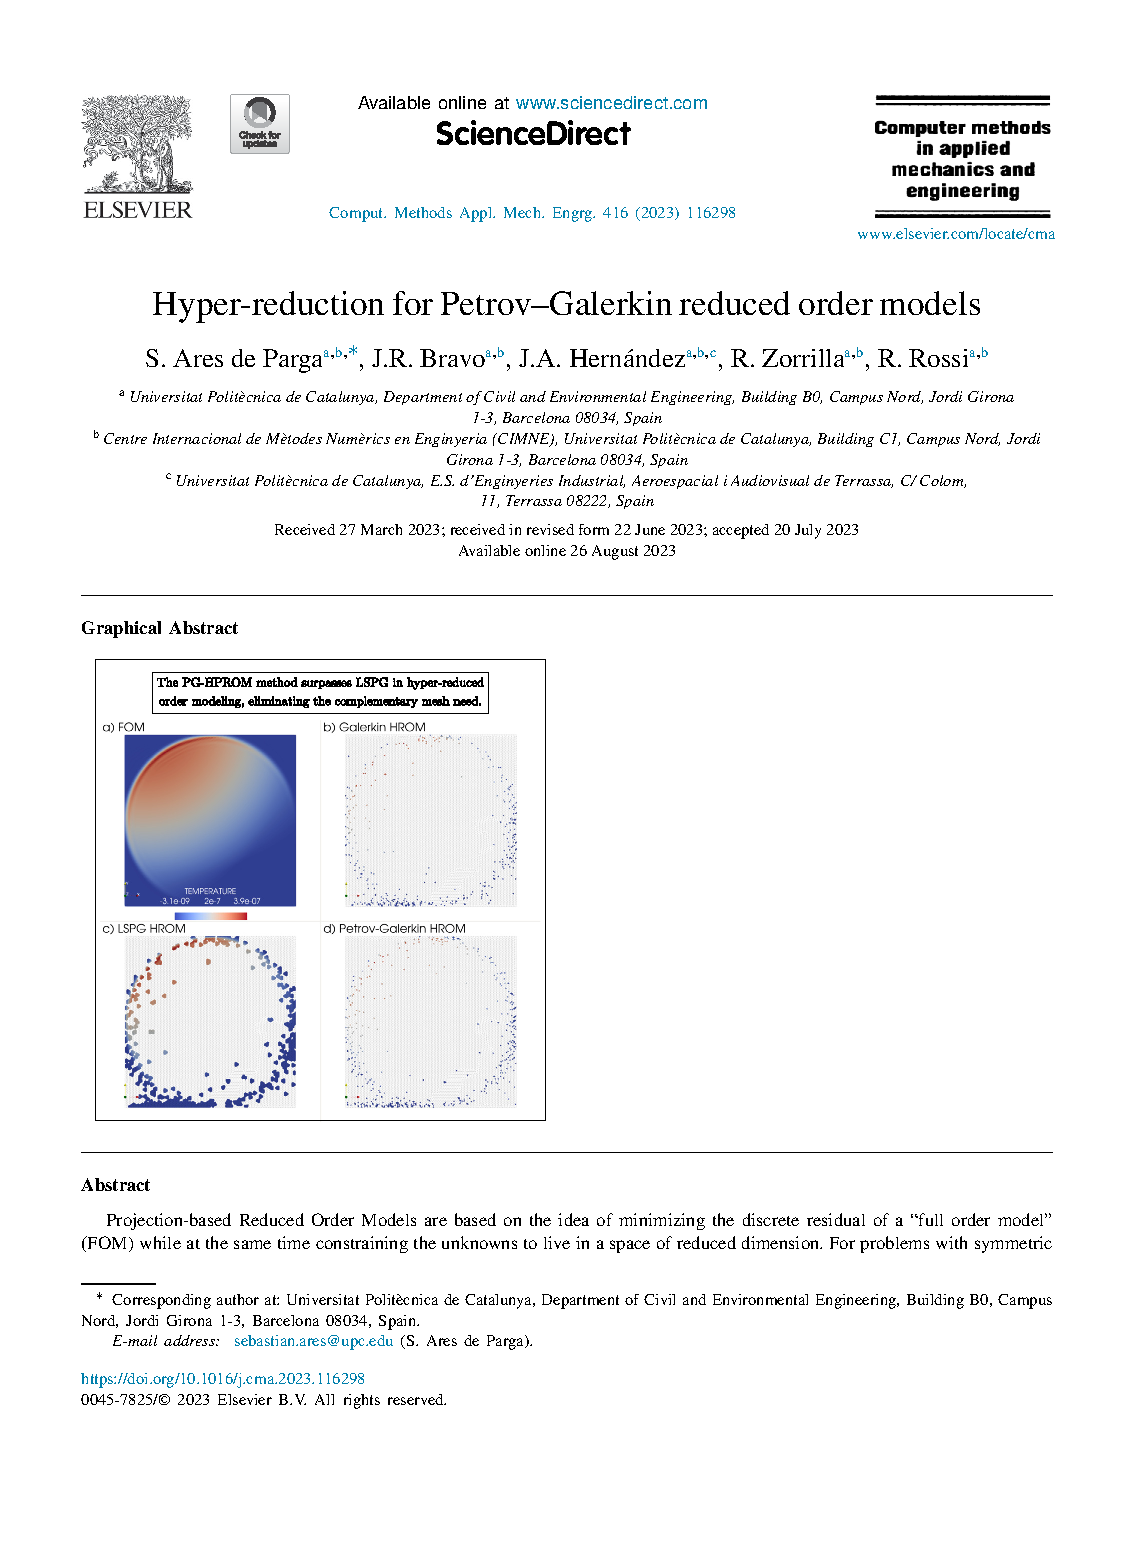
\includepdf[
  pages=-,
  pagecommand={},
  scale=0.92,
  delta=0 0,
  offset=32pt 0pt,
  turn=false
]{Papers/Hyper-reduction_for_Petrov–Galerkin_reduced_order_models.pdf}



